\icode{E-MD-SI-L2-261114-009}
如图所示，\(Oa\)、\(Ob\)和\(ad\)是竖直平面内三根固定的光滑细杆，\(O\)、\(a\)、\(b\)、\(c\)、\(d\)位于同一圆周上，\(c\)为圆周的最高点，\(O\)为最低点，\(O^\prime\)为圆心。每根杆上都套着一个小滑环，两个滑环从\(O\)点无初速释放，一个滑环从\(d\)点无初速释放，用\(t_1\)、\(t_2\)、\(t_3\)分别表示滑环沿\(Oa\)、\(Ob\)、\(ad\)到达\(a\)、\(b\)所用的时间，则下列关系正确的是\paren[]

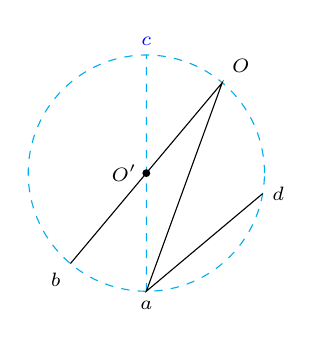
\begin{tikzpicture}[font=\scriptsize]
	\draw[dashed,cyan] (0,0) circle(1.5) (0,-1.5)--(0,1.5)node[above,blue]{\(c\)};
	\draw (-130:1.5)node[below left]{\(b\)}--(50:1.5)node[above right]{\(O\)}--(0,-1.5)node[below]{\(a\)}--++(40:{3*cos(50)})node[right]{\(d\)};
	\fill (0,0)node[left]{\(O^\prime\)} circle(.05);
\end{tikzpicture}
\begin{choices}
	\item \(t_1 = t_2 = t_3\)
	\item \(t_3 > t_1 > t_2\)
	\item \(t_1 < t_2 < t_3\)
	\item \(t_2 > t_1 = t_3\)
\end{choices}
\begin{answer}
    D\qquad 提示：
\end{answer}